\chapter{Social Navigation on Flickr \oldand Facebook}
\label{chapter:analysis}

In this chapter we'll look at the social navigation possibilities provided by
two large web sites with social characteristics\dash{}Flickr and Facebook.
Before we present the results of our investigation we'll describe the
methodology we used for dissecting the navigational structures of Flickr and
Facebook. We'll conclude this chapter, and the first part of our thesis, with
a discussion of our larger findings of how social navigation is used in
modern social web sites.

\section{Methodology}

The term \term{content analysis} is traditionally used to signify a
qualitative research method used in the social sciences.
\prequote[\p{18}]{krippendorff03}{defines it as}{%
  a research technique for making replicable and valid
  inferences from texts (or other meaningful matter) to the contexts of their
  use}
Even though such an analysis of the contents, meanings, or effects of
communication messages also have been utilized on the Web \citep{weare00}
it does not seem very well suited for understanding navigational mechanisms.

We turn to content analysis as the more pragmatic practice conducted within
the field of \term{information architecture}%
\sidenote{
  Information architecture can be explained as
  \begin{inparaenum}[(i)]
    \item the structural design of shared information environments,
    \item the combination of organization, labeling, search, and navigation
      systems within web sites and intranets,
    \item the art and science of shaping information products and experiences
      to support usability and findability, and
    \item an emerging discipline and community of practice focused on bringing
      principles of design and architecture to the digital landscape
      \citep[\p{4}]{morville06}.
  \end{inparaenum}
} hoping that it will help us get an better understanding of navigational
structures.
Content analysis is deployed as a technique by information architects for
helping them generate a sound and well structured web site architecture.
It's seen as a bottom-up process and
in its essence a content analysis should identify the various
relationships (or lack of correlation) between a web site's content items.
It consists of two phases:
\begin{inparaenum}[(i)]
  \item a collection of a representative sample of data and
  \item an analysis of this collected data
\end{inparaenum}
\citep[\pp{241}{243}]{morville06}.

Information architects are concerned with
the system's content and
\postquote[\p{94}]{batley07}{%
  need to move below the surface of the system
  interface to examine the system information itself}
We on the other hand are actually concerned with the system interface and
specifically its navigational structures. This creates a striking
contradiction as we're not interested in content unless it can help or
guide users during their navigation. We therefore have to adapt
both our inventory and analysis process accordingly.

\subsection{Inventory}

\term{Content inventory} is a technique for collecting data from web sites
in a structured manner. Its strength as a technique lies in its ability to
truly inform us about a web site's content \citep{wodtke02}. The process of
actually conducting a content inventory can be equally rewarding as the
resulting documents \citep{veen02}.

\subsubsection{Sampling}
\label{section:methodology.content.analysis.sampling}

Content inventories are often tedious and time consuming to perform.
\citet[\p{267}]{wodtke02} argues that every single bit of content needs to be
determined while \citet[\p{241}]{morville06} believes a representative sample
is sufficient.

The web sites that are interesting to look at in our research are vast and
loaded with enormous amounts of user generated content. An all-inclusive
approach to content gathering would simply be impossible in such situations.
As a remedy to this we've decided to ignore certain parts of web sites in our
content inventories since the scope of our research is limited to navigational
constructs, and only those of a social nature.

Our experience is that social navigation and more static navigation are
intermixed all over web sites. Often one have to use non-social forms of
navigation before social navigational options appear. Thus we could not simply
ignore navigational aims which were non-social in our content inventory phase.
We did however eliminate the following parts of web sites under investigation:

\begin{enum}
  \iterm{Administrative sections} where users can change their profiles or set
    their preferences\dash{}a private and asocial endeavour.
  \iterm{Help pages} where \abbr{FAQ}s, guides, and instructions are presented
    in a static manner.
  \iterm{Legal information} including terms of service, privacy policies, and
    copyright notices.
  \iterm{Content generation} facilities like uploading, categorizing, and
    editing photos, commenting, posting items, and so on.%
    \sidenote[-10]{
      While there is no question about the usefulness of such content for
      providing social navigation possibilities we've found few examples where
      social navigation is used in the content generation phases itself.
      There is however a few exceptions, like applying tags (see
      \sectionref{background.social.navigation.applied.forms.tagging.sharing}
      for details).
    }
  \iterm{Advertisements} from third party providers.
\end{enum}

In addition to eliminating certain form of web pages we synthesized abstract
page representations by introducing variables. Take for example a typical
social network site. There are from thousands to several millions of
profile pages. In context of what navigational options these pages present to
us they are all essential similar. So we could introduce a variable called
\var{user-name}%
\sidenote[-5]{
  The variable notation with a dollar (\$) prefix is inspired from
  variable usage in \abbr{UNIX} shell scripting \citep[\p{88}]{kernighan84}.
}
and thereby describe all potential profile pages as:
\val{Profile of \var{user-name}},

We would however have to make sure that the one page we used in our inventory
to represent the abstract notion of a profile page was representative. To
exemplify, say that a profile page included a stream of the 10 most recent
actions your friends had conducted. If the user of our collected profile page
had zero friends we would lack the navigational opportunities such a stream
could give in our inventory. Therefore we used only pages which provided
all possible forms of navigation as basis for abstraction.

\subsubsection{Approach}

We started out on the first page that was given us when entering the web site
under investigation. From there we stepped trough each page of the web site
by following all navigational hyperlinks provided on individual pages.
We did not however frequent a web site in its entirety, but bearing in mind
our sampling constraints and abstractions we frequented the site to full
coverage. We stopped browsing a particular page if it%
\sidenote{
  Either the exact same page or a page deemed to be the same by our
  variable driven abstraction method.
}
had been previously been inventoried. During the course of this browsing
each page was noted down in a table with the following characteristics:

\begin{enum}
  \iterm{Identifier} of numerical and hierarchical form where page with id
    4.3.1 is the first child of a page with id 4.3, representing its place in
    the navigation structure. The first page was given an id of \val{0},
    its first descendant an id of \val{1} and so on.
  \iterm{Page title} as a description of what the page contains. Some of the
    web site's we surveyed had a slight ambiguity of title usage. In these
    cases we decided to collect the most representative sample.%
    \sidenote{
      A choice between the \code{<title>} element in the \code{<head>}
      of the \abbr{HTML} document and the \code{<h1>} top level heading
      in-line the \code{<body>} portion of the document was made.
    }
    If this resulted in unsatisfactory results we created a new title using
    the best of our abilities to make it as clear and descriptive as possible.
  \iterm{Link name} is either the textual name or a description of the
    contents (i.e. a graphical representation) of the hyperlink that was
    utilized to navigate to this very page.
  \iterm{Link location} as a description of the spatial position
    (for example: global navigation, content area, right sidebar) of the
    hyperlink used to navigate to this page.
  \iterm{Page \abbr{URL}} as an identifier for the page we visited.
\end{enum}

The result was a table representing a web site's various pages and the
navigational relationships amongst them.

While we took note of the \abbr{URL} of each page we've decided not to display
this information. We're not convinced of its usefulness in light of
navigation and therefore for brevity's sake omitted them. We did however use
them in our inventory process as a way to identify previously collected pages.

In a traditional content inventory other characteristics
is usually collected.%
\sidenote{
  For an example of more traditional collection methods
  see \citet[\p{269}]{wodtke02}.
}
As we described earlier we're only concerned with the navigational parts of
web pages. We opted to only record what we found to be useful for this
purpose. This lead to a situation where we were collecting more information
about site structure than the attributes of a site's content\dash{}as an
information architect usually would do.

\subsection{Analysis}

An analysis of the collected content follows after an inventory phase is
completed. Typically information architects use content analysis for
making decisions on what and how to improve an existing web site's content
architecture. With such an aim they look for patterns and relationships when
analyzing their content inventory. These patterns and relationships will then
suggest groupings and connections amongst separate content items
\cite[\p{243}]{morville06}.

\subsubsection{Approach}
Since our focus were dissimilar compared to that of most information
architects' we've had to tailor the analysis process to best help us discover
and understand patterns of social navigation in web sites. Analyzing content
inventories for such means is as far as we know not conducted before. We were
therefore exploring unknown waters and had to adapt our method as we
went about with our analysis.

We started with our impressions from the content inventory%
\sidenote{
  As stated earlier the process of conducting a content inventory is not only
  beneficial just because of the resulting documentation one creates of a web
  site. People conducting content inventories tends to get deeply informed
  about a web sites content and structure after having exhaustively recorded
  large parts of it. 
}
and based our discussion on the findings we regard most conspicuous in
relation to social navigation. During the resulting discussion we
referenced the relevant pages recorded in our content inventory by their
identifiers.

\section{Results}

This section includes a survey and analysis of the most interesting
data we've collected in our inventory phase of a content analysis
of two well known web sites. The inventory results can be found in its whole
in \appendixref{content.inventory}. When we're referencing to \abbr{ID}s we're
using the identifier in the tables found at the specified pages.

\subsection{Social Navigation on Flickr}
\label{section:analysis.flickr}

Flickr is a photo sharing site which are known to be on the cutting edge when
it comes to enabling new and innovating features in its domain. Flickr has a
quite peculiar history as it started out as a massively multi player online
game. An environment for photo sharing within the game was added in 2004 which
quickly became more popular than the game itself. The focus of the company was
shifted and their new photo sharing community was bought by Yahoo! Inc. in
March 2005 \citep[\p{257}]{livingston07}.

This subsequent
analysis of Flickr was carried out as a registered user. One has to be
registered for interacting with the site in such a way that one leaves
persistent traces. The site has a open nature enabling anonymous access
to the majority of content.

\subsubsection{Thumbnails}

Already on the welcome page (\figureref{scrsh.flickr.welcome})
we're finding navigation links that are social of
nature. Four thumbnails functions as sample of the most recently uploaded
photos by other members of the community and four thumbnails samples the
latest photos by your friends.
One can either navigate straight to
a detailed page for each particular photo by clicking on the respective
thumbnail \flickrref{6}
or the profile of the uploader by clicking on their user
name \flickrref{7}. Such thumbnails
with minimal meta data (the uploader) are prevalent all over Flickr. Of the
120 pages we collected in our content inventory 26 of them
\begin{sparkline}{3}
  %Name  Size Percent Unit
  %All   120  100     1
  %Thumb  26   22      .22
  \sparkspike .25  1
  \sparkspike .75  .22
\end{sparkline}
contained thumbnails. Most of these thumbnails
are giving users incentives to navigate using social means.%
\sidenote[-3]{%
  Apart from the few pages that only show a
  stream of your own thumbnails when you're browsing your
  own photos by various methods.
}
Which photos these thumbnails portray is dynamic. That is to say that other
users' actions\dash{}uploading a photo, tagging a photo, taking a photo with a
specific camera, collecting photos into sets, and adding photos to a certain
group\dash{}all determine the navigational choices you as a user is
presented with. A typical example of passive and indirect social navigation
with both implicit and explicit transfer of advice.

\subsubsection{Meta-data}

\begin{figure}
  \captionstyle{\raggedright}
  \begin{whole}
    \begin{minipage}[t]{0.475\wholewidth}
      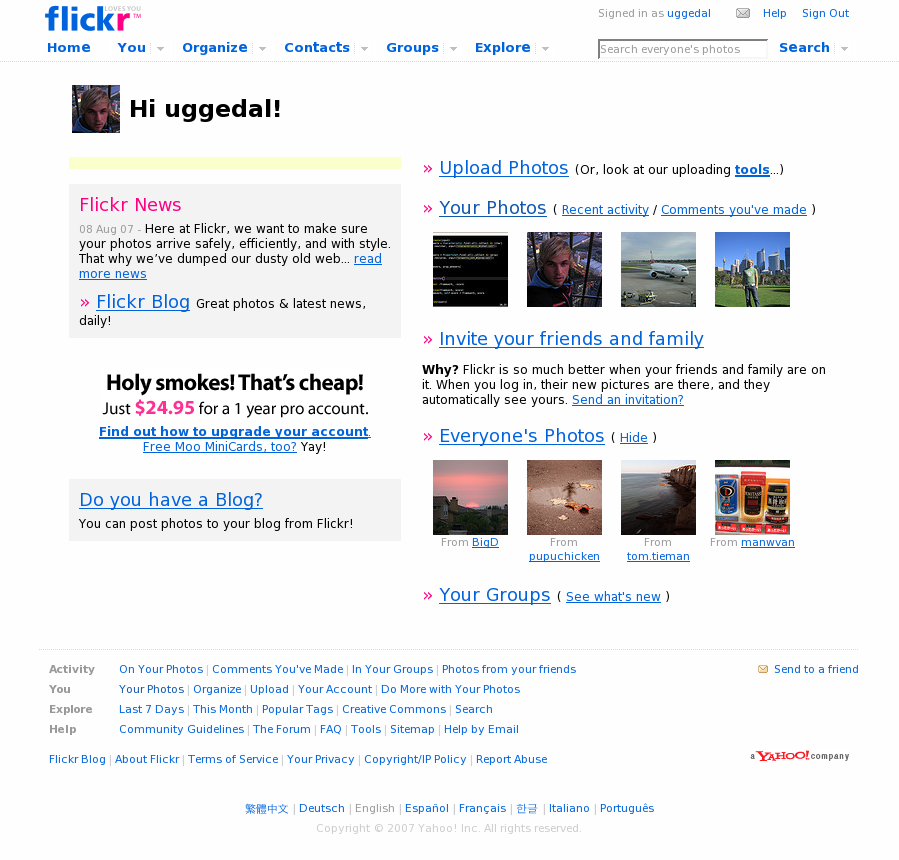
\includegraphics[width=\textwidth]{scrsh_flickr_welcome}
      \caption[Flickr Welcome Page]{%
         The welcome page of Flickr,
         retrieved October 16, 2007, from \url{http://flickr.com}}
      \label{figure:scrsh.flickr.welcome}
    \end{minipage}
    \hfill
    \begin{minipage}[t]{0.475\wholewidth}
      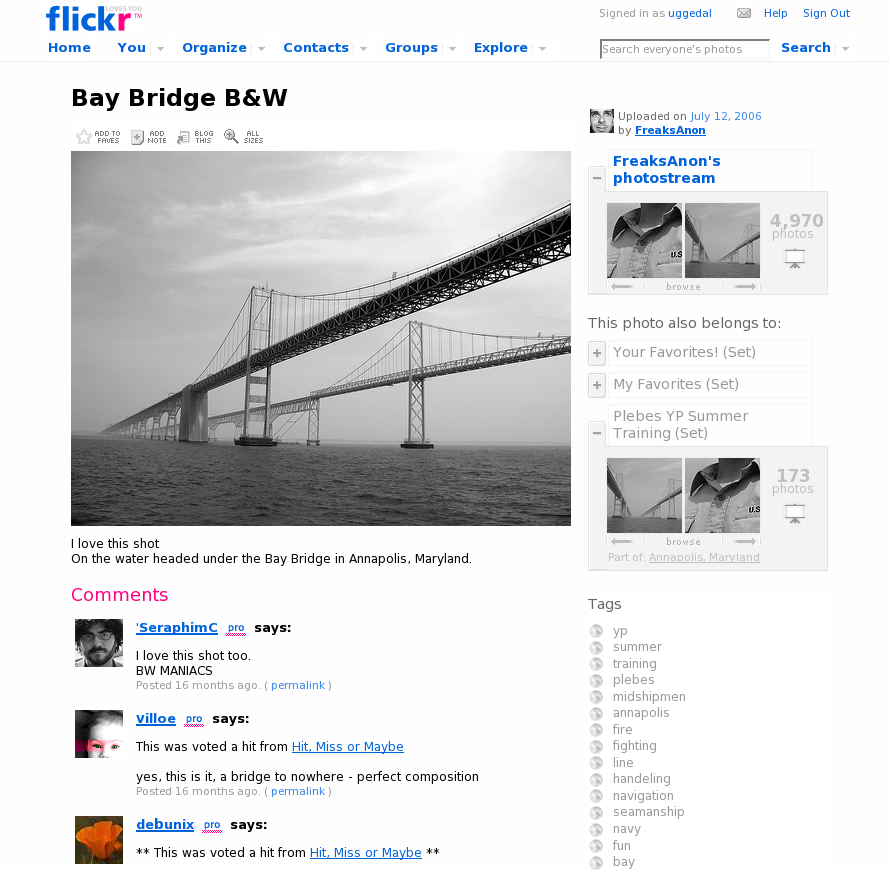
\includegraphics[width=\textwidth]{scrsh_flickr_photo_detail}
      \caption[Flickr Photo Detail Page]{%
         A photo detail page on Flickr,
         retrieved October 26, 2007, from
         \url{http://flickr.com/photos/benbengraves/187609810}}
      \label{figure:scrsh.flickr.photo.detail}
    \end{minipage}
  \end{whole}
  \normalcaption
\end{figure}

\sidefigure[Flickr Photo Meta-data]{%
  Photo meta-data on Flickr,
  retrieved October 28, 2007, from
  \url{http://flickr.com/photos/benbengraves/187609810/}
  \label{figure:scrsh.flickr.photo.detail.metadata}
}{%
  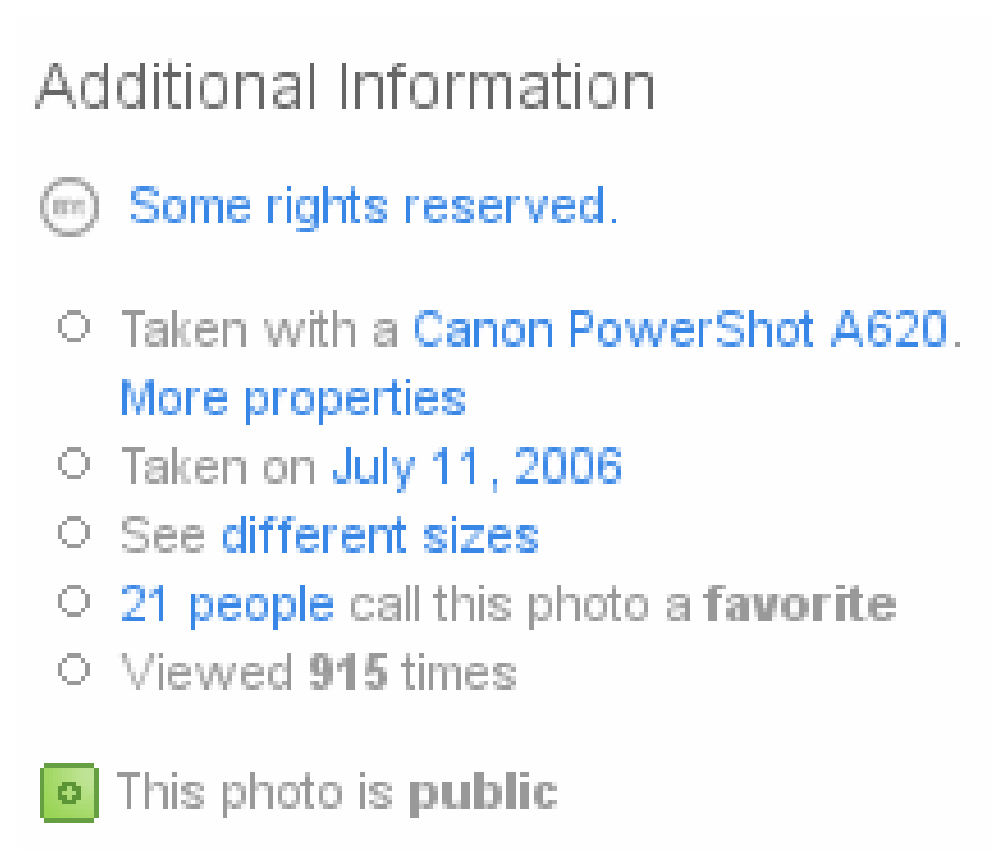
\includegraphics[width=0.9\marginparwidth]{scrsh_flickr_photo_metadata}
}

We arrive on a photo detail page \flickrref{1.1} as in
\figureref{scrsh.flickr.photo.detail}
if we utilize one of these thumbnails for navigation. In addition to comments
on the photo we find meta-data as in 
\figureref{scrsh.flickr.photo.detail.metadata}
Meta-data include the date the photo was taken, the manufacturer and the model
of the camera that was used which are all so called \term{Exif}%
\sidenote[-9]{%
  Short for Exchangeable Image File\dash{}a specification for an image
  file format used in digital cameras.
}
data. Flickr utilize this data by enabling navigation based both on the
dates a picture was taken and by camera make and model\dash{}social navigation
with implicit advice. Say you're trying to
find a picture from your home town on a particularly beautiful summer day. By
using date of picture taking based navigation coupled with tags or
geographical data (which both will be discussed shortly) you're probably
increasing you chances of finding what you want. Camera make information could
also be useful when looking at the quality of pictures taken with certain
cameras before purchasing one yourself.

\subsubsection{Folksonomy}
Of most importance
for Flickr, and indeed what makes Flickr a folksonomy, is its tagging
abilities. Caterina Fake, co-founder of Flickr, explains its importance as
\postquote[\p{261}]{livingston07}{%
  Tagging really revolutionized the way the product behaved}
All registered user can label anyone's photos by applying such short
descriptive tags. This collaborative process lay the ground work for other
user's ability to easily browse photos by topic\dash{}a form of indirect and
passive social navigation where advice are explicitly given.
\figureref{scrsh.flickr.tagcloud}
exemplifies how the user generated data trough tagging \flickrref{5}
can be used as a navigational aid. A tag cloud is used to visualize the
popularity (and thereby importance) of the individual tags. The larger the
tag title, the more frequent the tag has been applied to photographs.

\begin{figure}
  \begin{whole}
    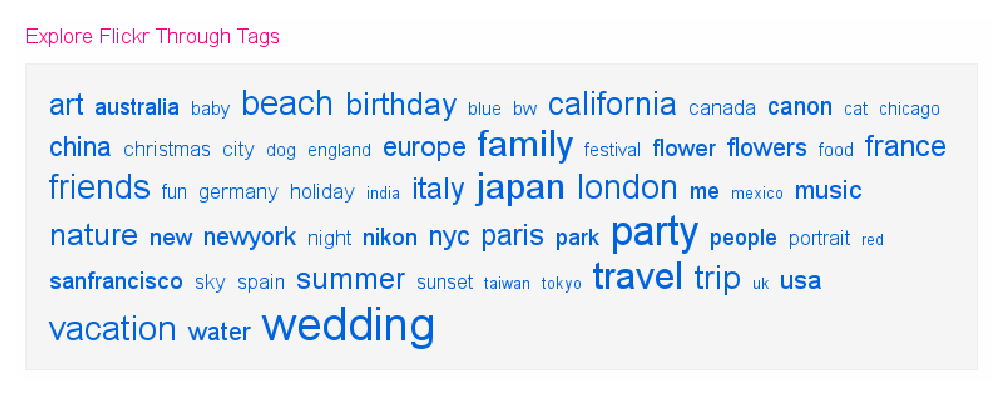
\includegraphics[width=\wholewidth]{scrsh_flickr_tagcloud}
    \caption[Flickr Tag Cloud]{%
       Tag cloud on Flickr,
       retrieved November 1, 2007, from \url{http://flickr.com/explore}}
    \label{figure:scrsh.flickr.tagcloud}
  \end{whole}
\end{figure}

\term{Tag clustering} was released in the fall of 2005 \citep{butterfield05}
as a way to easier see the relationships between separate tags. For any given
tag a cluster of three related tags is generated and displayed
\flickrref{5.6.1.2} to users when
they are browsing as seen in \figureref{scrsh.flickr.tagcluster}.
Flickr algorithmically generates these listings based on what tags users tend
to use together for labeling a photo.

\begin{figure}
  \begin{whole}
    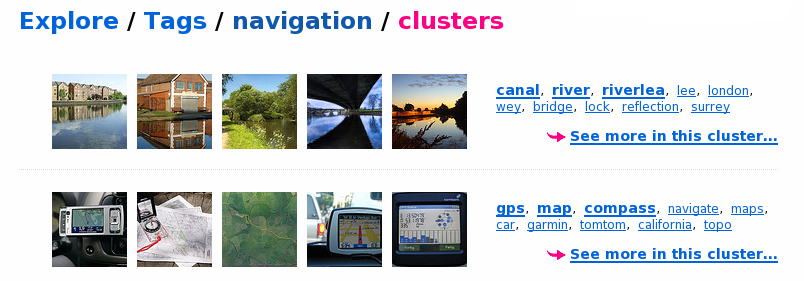
\includegraphics[width=\wholewidth]{scrsh_flickr_tagcluster}
    \caption[Flickr Tag Cluster]{%
       Tag cluster on Flickr,
       retrieved November 19, 2007, from
       \url{http://flickr.com/photos/tags/navigation/clusters/}}
    \label{figure:scrsh.flickr.tagcluster}
  \end{whole}
\end{figure}

Tagging is a very flexible approach only hindered by users' imagination. In
the early days of Flickr there was no support for geographical data. Users
soon found a remedy for this by tagging photos with the longitude and
latitude of the place where they were taken.
By using the same technology we're using in our prototype
application (see \sectionref{selection.stack.client.platform} for details)
they were able to integrate Google Maps%
\sidenote{
  Google Maps, an online interactive geographical map of the world ,can be
  found at \url{http://maps.google.com}.
} in Flickr, enabling user's to place their photos on a map and automatically
generate geographical coordinate tags.%
\sidenote[2]{
  More info about \term{geotagging} in the early days of Flickr can be found
  in the remains of the Flickr Geotagging group, available at
  \url{http://flickr.com/groups/geotagging/}.
}

\subsubsection{Geographical data}

In late August 2006 Flickr introduced geotagging abilities
\citep{butterfield06a} by integrating mapping aspects from Yahoo! Maps.%
\sidenote[3]{
  Yahoo! Maps, a service similar to Google Maps, have its home at
  \url{http://maps.yahoo.com}.
}
Users could now place their photos on a
map to signify where they were captured without resorting to clever hacks of
the standard tagging system.

\figureref{scrsh.flickr.geotagged} shows how one of the authors photos are
placed on a map \flickrref{1.1.6}.
One can then cycle trough the adjacent photos of other users
that are interesting or recently published.
What we see here is indirect social navigation where the advice is explicitly
given. When a user places his photo geographically on a map he makes available
navigational choices for other users who for some reason are interested in
that particular geographical area. Such visualizations of geographic
navigation clues are a good example of social texture.

\begin{figure}
  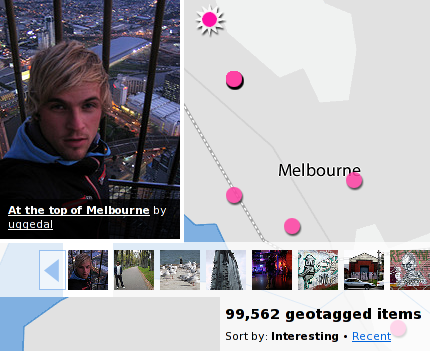
\includegraphics[width=0.8\textwidth]{scrsh_flickr_geotagged}
  \caption[Flickr Geotagging]{%
     Geotagging on Flickr,
     retrieved March 3, 2008, from
     \url{http://flickr.com/photos/uggedal/261824261/map/?view=everyones}}
  \label{figure:scrsh.flickr.geotagged}
\end{figure}

\subsubsection{Interestingness}
\label{section:analysis.flickr.interestingness}

The concept of \term{interestingness} was introduced by Flickr during
the same time tag clustering was unveiled \citep{butterfield05}.

Interestingness is a rating of how interesting a photograph is deemed to be.
Interestingness is based on
how many views the photograph has, how many users who have favored the
photograph, and how many comments the photograph has. Favoring have the
highest weight, comments medium weight, and views the least weight
in the algorithm that generates the interestingness rating \citep{dean08}.
Users are not aware of the score of a particular photograph's interestingness,
but the highest rated photographs are available trough the \q{Explore} part of
Flickr
(\flickropenref{5.3}
\flickropenref{5.4}).

The interestingness system is a great example of passive and indirect social
navigation. Based on the behavior of other users the more interesting photos
are made more visible in Flickr's interface. Flickr can be seen as a
collaborative filtering system which uses implicit and explicit ratings.
When a user leaves a comment on a photo the aim is likely to voice his
reactions to the picture, and not vote the picture down or up. Page views
are also implicit of nature while favoring are explicitly given by users.

Interestingly Flickr uses
collaborative filtering without personalization of it's recommendations and
rather gives the whole population similar recommendations.
The use of interestingness seem
to have worked well for Flickr as users are trying hard to make their photos
receive higher interestingness scores.
As of this writing a patent on interestingness is pending
\citep{butterfield06b}.

\subsection{Social Navigation on Facebook}
\label{section:analysis.facebook}

Facebook is a social network site which started as a service only available
for Harvard students in February of 2004. Within the same month Facebook was
opened up for students at several other universities in the \abbr{US}. More
universities and colleges were supported before Facebook opened up it
doors for high-school students in September of 2005 \citep{cassidy06}.
Anyone\dash{}student or not\dash{}was allowed access in
September of 2006 \citep{abram06}.
Facebook has seen an enormous growth and are today the largest social network
in some countries (see
\sectionref{background.sociality.the.social.web.social.network.sites}
for details).

The following analysis was carried out as an authenticated user of Facebook.
Most of Facebook's content is only available for registered users. Each user's
privacy settings also regulates how openly available content is.

\subsubsection{News feed}
\label{section:analysis.facebook.news.feed}

\begin{figure}
  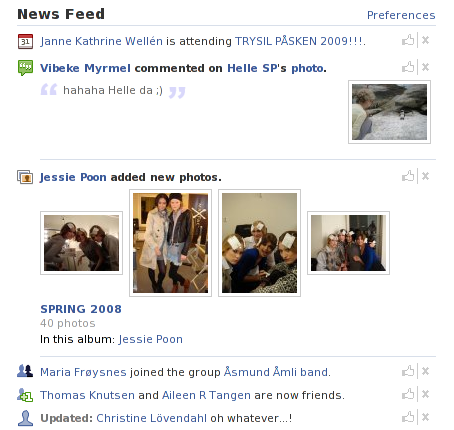
\includegraphics[width=0.9\textwidth]{scrsh_facebook_news_feed}
  \caption[Facebook News Feed]{%
     Author's news feed on Facebook,
     retrieved March 26, 2008, from \url{http://www.facebook.com/home.php}}
  \label{figure:scrsh.facebook.news.feed}
\end{figure}

The landing page when you log in to Facebook after having configured your
account is the \q{News Feed} \facebookref{0}.
The news feed shows the recent activities your
friends have conducted. This eliminates the tedious process of checking every
profile page of your friends to keep on top of what they're up to.
The feed shows a list of items, each representing a type of activity. As
shown in \figureref{scrsh.facebook.news.feed}
these activities are distinguished by an
icon and presented chronologically. The data presented in the news feed are an
aggregation of every friend's \q{Mini-Feed} located on their profile page
\facebookref{1} as seen in \figureref{scrsh.facebook.profile}.

\begin{figure}
  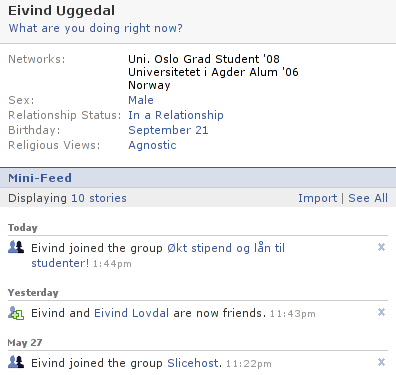
\includegraphics[width=0.9\textwidth]{scrsh_facebook_profile}
  \caption[Facebook Profile]{%
     Author's profile page on Facebook,
     retrieved May 30, 2008, from
     \url{http://www.facebook.com/profile.php?id=903795175}}
  \label{figure:scrsh.facebook.profile}
\end{figure}

The news feed enables social navigation\dash{}all
navigational choices the feed provides
trough representations of activity are constructed as a by-product of
other people's actions. When you select to attend an event, join a group,
post a photo, change your relationship settings, befriend a person, post a
comment on a wall or photo, or update your profile information your action
is added to the feed. The navigation presented by the feed
is therefore indirect and passive social navigation provided by implicit
feedback\dash{}providing no additional overhead for the advice provider.

\subsubsection{Hyperlink sharing}

Facebook have an interesting feature that makes hyperlink sharing easier for
it's users. When one are posting a comment on a the wall of a person
\facebookref{1.19.1},
group
\facebookref{1.1.3.1.1.9},
or event
\facebookref{1.1.3.2.1.9}
one can provide a \abbr{URL}. By providing such a hyperlink to a
third party web page Facebook extracts an excerpt of the linked page with
optional graphics as seen in \figureref{scrsh.facebook.wall.link}. Since the
recipient of a message with a hyperlink can respond to the advice provider
we're witnessing active and direct social navigation. This
improved \abbr{URL} handling was envisioned by
\citet[\p{811}]{dieberger97}.

\begin{figure}
  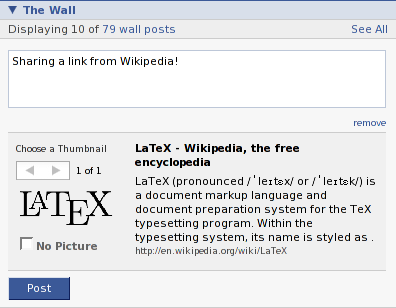
\includegraphics[width=0.8\textwidth]{scrsh_facebook_wall_link}
  \caption[Facebook Hyperlink Sharing]{%
     Sharing of hyperlinks on Facebook,
     retrieved June 2, 2008, from
     \url{http://www.facebook.com/profile.php?id=903795175}}
  \label{figure:scrsh.facebook.wall.link}
\end{figure}

\subsubsection{Photo tagging}

Photos on Facebook can be tagged \facebookref{1.19.1} like those on Flickr.
But as you can see in \figureref{scrsh.facebook.photo.tagging} one are
tagging with people as identifiers on Facebook instead of keywords as on
Flickr. We are
therefore not witnessing a folksonomy on Facebook. Photo tagging on Facebook
can be used as a means of navigating photos of particular individuals or
navigating towards people based on photos with various taggings of
individuals.

Photo tagging can therefore be seen as passive and indirect social navigation
where advice is given explicitly.
Navigational advice is made available for future users when they stumble upon
a photo with person tags, person tags in news feeds, or navigates photos by a
certain tagged person.

\begin{figure}
  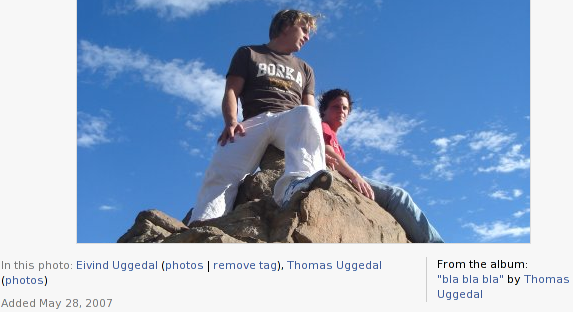
\includegraphics[width=0.9\textwidth]{scrsh_facebook_photo_tagging}
  \caption[Facebook Photo Tagging]{%
     Photo tagging on Facebook,
     retrieved June 2, 2008, from
     \url{http://www.facebook.com/photo.php?pid=177290&id=579356186}}
  \label{figure:scrsh.facebook.photo.tagging}
\end{figure}

\section{Discussion}

Trough our study of Flickr and Facebook we've gotten an impression of how
social navigation is used in modern web sites. We'll discuss our most
interesting findings in the next sections.

\subsection{No explicit design for social navigation}

It does not seem like the designers of social web pages design for social
navigation explicitly. There seem to be a trend of designing for social
interaction. As we discussed in
\sectionref{background.sociality.the.social.web.ggg}, the inventor of the Web
now sees social relationships as a highly important part of the modern web.
In addition we've seen in
\sectionref{background.sociality.the.social.web.social.network.sites}
that social network sites have become very popular amongst web citizens.

An implicit by-product of such a design approach seems to be
the creation of several forms of social navigation constructs.
We base this observation on our studies of two large social web sites
(see \chapterref{analysis} for details)
in addition to cursory observations from other social web sites.

\subsection{Social navigation have become mainstream}

We were able to locate navigational mechanisms which could be considered
social navigation in all the web sites we studied. While our view of the
modern web surely is uncomplete, we take this as a sign for an increased use
of social navigation. Social navigation seems to have become mainstream.

The reasons for this increased usage can be many. We think the most dominant
factor is the high focus on creating web sites where social interaction is
supported. As described earlier, social navigation is then implicitly created
when one designs web sites with such a focus.

\subsection{Social navigation advice is given by peers}

An overlying theme of the forms of social navigation we found in the wild were
that it was created by equal peers. The constructs for enabling social
navigation are created by the web site creators. But the data that
enables navigational choices of a social nature are created by other
users\dash{}by the community.

We therefore purpose that navigational advice have to
be given by peers to be considered social navigation,
whether indirect or direct, explicit or implicit.
In other words
navigational advice have to be given by individuals on the same horizontal
level as yourself. This means that navigational advice given by web editors
and web designers\dash{}people vertically superior to yourself\dash{}can not
be considered true social navigation.

